\documentclass[12pt,letterpaper]{article}
\usepackage{graphicx,textcomp}
\usepackage{natbib}
\usepackage{setspace}
\usepackage{fullpage}
\usepackage{color}
\usepackage[reqno]{amsmath}
\usepackage{amsthm}
\usepackage{fancyvrb}
\usepackage{amssymb,enumerate}
\usepackage[all]{xy}
\usepackage{endnotes}
\usepackage{lscape}
\newtheorem{com}{Comment}
\usepackage{float}
\usepackage{hyperref}
\newtheorem{lem} {Lemma}
\newtheorem{prop}{Proposition}
\newtheorem{thm}{Theorem}
\newtheorem{defn}{Definition}
\newtheorem{cor}{Corollary}
\newtheorem{obs}{Observation}
\usepackage[compact]{titlesec}
\usepackage{dcolumn}
\usepackage{tikz}
\usetikzlibrary{arrows}
\usepackage{multirow}
\usepackage{xcolor}
\newcolumntype{.}{D{.}{.}{-1}}
\newcolumntype{d}[1]{D{.}{.}{#1}}
\definecolor{light-gray}{gray}{0.65}
\usepackage{url}
\usepackage{listings}
\usepackage{color}

\UseRawInputEncoding
% from lshort.pdf
\usepackage{verbatim}
% includes comment env
\definecolor{codegreen}{rgb}{0,0.6,0}
\definecolor{codegray}{rgb}{0.5,0.5,0.5}
\definecolor{codepurple}{rgb}{0.58,0,0.82}
\definecolor{backcolour}{rgb}{0.95,0.95,0.92}

\lstdefinestyle{mystyle}{
	backgroundcolor=\color{backcolour},   
	commentstyle=\color{codegreen},
	keywordstyle=\color{magenta},
	numberstyle=\tiny\color{codegray},
	stringstyle=\color{codepurple},
	basicstyle=\footnotesize,
	breakatwhitespace=false,         
	breaklines=true,                 
	captionpos=b,                    
	keepspaces=true,                 
	numbers=left,                    
	numbersep=5pt,                  
	showspaces=false,                
	showstringspaces=false,
	showtabs=false,                  
	tabsize=2
}
\lstset{style=mystyle}
\newcommand{\Sref}[1]{Section~\ref{#1}}
\newtheorem{hyp}{Hypothesis}

\title{Problem Set 2}
\date{Due: October 16, 2022}
\author{Applied Stats/Quant Methods 1}

\begin{document}
	\maketitle
	
	\begin{comment}
	\section*{Instructions}
\begin{itemize}
	\item Please show your work! You may lose points by simply writing in the answer. If the problem requires you to execute commands in \texttt{R}, please include the code you used to get your answers. Please also include the \texttt{.R} file that contains your code. If you are not sure if work needs to be shown for a particular problem, please ask.
	\item Your homework should be submitted electronically on GitHub.
	\item This problem set is due before 23:59 on Sunday October 16, 2022. No late assignments will be accepted.
	\item Total available points for this homework is 80.
\end{itemize}

	\end{comment}
	
	\vspace{.5cm}
	\section*{Question 1 (40 points): Political Science}
		\vspace{.25cm}
	The following table was created using the data from a study run in a major Latin American city.\footnote{Fried, Lagunes, and Venkataramani (2010). ``Corruption and Inequality at the Crossroad: A Multimethod Study of Bribery and Discrimination in Latin America. \textit{Latin American Research Review}. 45 (1): 76-97.} As part of the experimental treatment in the study, one employee of the research team was chosen to make illegal left turns across traffic to draw the attention of the police officers on shift. Two employee drivers were upper class, two were lower class drivers, and the identity of the driver was randomly assigned per encounter. The researchers were interested in whether officers were more or less likely to solicit a bribe from drivers depending on their class (officers use phrases like, ``We can solve this the easy way'' to draw a bribe). The table below shows the resulting data.

%\newpage
\begin{table}[htb!]
	\centering
	\begin{tabular}{l | c c c }
		& Not Stopped & Bribe requested & Stopped/given warning \\
		\\[-1.8ex] 
		\hline \\[-1.8ex]
		Upper class & 14 & 6 & 7 \\
		Lower class & 7 & 7 & 1 \\
		\hline
	\end{tabular}
\end{table}

\begin{enumerate}

	\item [(a)]
	The $\chi^2$ test statistic is calculated as follows:\\
	%\vspace{7cm}
	
	Read in the data as a matrix.
	\lstinputlisting[language=R, firstline=61, lastline=61]{PS02.R}  

	Calculate the expected values, then calculate the difference between the observed 
	and expected values for each sub-category.  Calculate the contribution to the 
	$\chi^2$ statistic. 
	\begin{description}
	  \item[expected] number in class * number of outcomes / total number
	  \item[difference] observed - expected
	  \item[contribution] difference$^2$/expected) 
	 \end{description}
		
		For example, for the sub-category `Upper Class' and `Not Stopped':
	
	\begin{table}[htb]
		\centering
		\begin{tabular}{l | l}
			\multicolumn{2}{c}{Upper Class, Not Stopped} \\
			\\[-1.8ex] 
			\hline \\[-1.8ex]
			observed  &  14  \\
			expected  &  13.5 = (27 * 21 / 42)\\
			difference  &  0.5  = (14 - 13.5)\\
			chi sq contribution  &  0.0185  = (0.5 )$^2$ / 13.5\\
			
		\end{tabular}
	\end{table}
	
	\lstinputlisting[language=R, firstline=71, lastline=99]{PS02.R}  

	\item [(b)]
	The p-value from the test statistic is calculated as follows.  
	If $\alpha = 0.1$, we cannot reject the null hypothesis that both subgroups
	are from the same population (i.e. the difference in experience is not 
	statistically significant).\\
	
	\lstinputlisting[language=R, firstline=119, lastline=119]{PS02.R}  
	
	\begin{verbatim}
	  The p-value is 15.02%, alpha is 10%
	   We cannot reject the null hypothesis that the two sets are from the
same population
	   1 observed cell(s) with less than 5 values
	\end{verbatim}

  The observed and expected values are shown in Figure~\ref{fig:obs_exp}	
	\begin{figure}
		  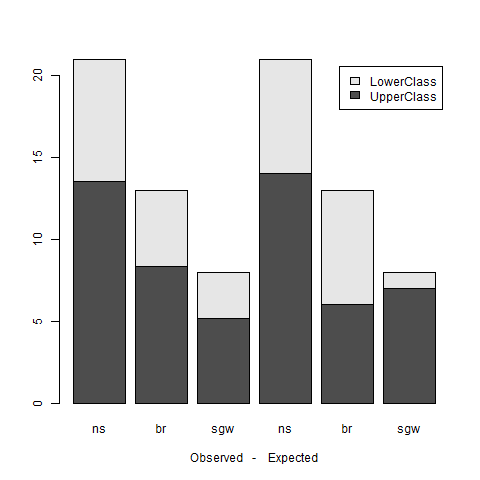
\includegraphics{graphics/obs_exp.png}
		  \caption{Observed vs Expected values for traffic stop. ns = Not Stopped; br = Bribe Requested; sgw = Stopped Given Warning}\label{fig:obs_exp}
	\end{figure}

  The results of the builtin \texttt{R} chisq.test function are as follows:
  \begin{verbatim}
  
	Pearson's Chi-squared test

  data:  observed
  X-squared = 3.7912, df = 2, p-value = 0.1502
\end{verbatim}

%	\newpage
	\item [(c)] The standardized residuals are set out in Table~\ref{tab:StandardisedResiduals}:
	%\vspace{1cm}

	
% Table created by stargazer v.5.2.3 by Marek Hlavac, Social Policy Institute. E-mail: marek.hlavac at gmail.com
% Date and time: Mon, Oct 10, 2022 - 20:14:46
\begin{table}[h] \centering 
  \caption{Standardised Residuals} 
  \label{StandardisedResiduals} 
\begin{tabular}{@{\extracolsep{5pt}} cccc} 
\\[-1.8ex]\hline \\[-1.8ex] 
 & NotStopped & BribeRequested & StoppedGivenWarning \\ 
\hline \\[-1.8ex] 
UpperClass & $0.32$ & $$-$1.64$ & $1.52$ \\ 
LowerClass & $$-$0.32$ & $1.64$ & $$-$1.52$ \\ 
\hline \\[-1.8ex] 
\end{tabular} 
\end{table}  

	
	%\vspace{7cm}
	\item [(d)] How might the standardized residuals help you interpret the results?  

    The biggest contribution to the residuals was from the `Bribe Requested' variable - 
    fewer upper class individuals were expected to hand over bribes.  The difference 
    between the two groups appears to be a combination of fewer upper class drivers
    being expected to hand over bribes and more of them being given a warning instead 
    the opposite outcome occuring for lower class drivers.

    We are not rejecting the null hypothesis, so we are concluding that there may
    not be any significant relationship between class and the outcomes experienced 
    during traffic stops.  The combined effect from the diffent experiences of the two 
    groups was not enough to convince us that class predicts whether or not a driver
    is asked for a bribe.
    
  
\end{enumerate}

\newpage

\section*{Question 2 (40 points): Economics}

Chattopadhyay and Duflo were interested in whether women promote different policies than men.\footnote{Chattopadhyay and Duflo. (2004). ``Women as Policy Makers: Evidence from a Randomized Policy Experiment in India. \textit{Econometrica}. 72 (5), 1409-1443.} Answering this question with observational data is pretty difficult due to potential confounding problems (e.g. the districts that choose female politicians are likely to systematically differ in other aspects too). Hence, they exploit a randomized policy experiment in India, where since the mid-1990s, $\frac{1}{3}$ of village council heads have been randomly reserved for women. A subset of the data from West Bengal can be found at the following link: \url{https://raw.githubusercontent.com/kosukeimai/qss/master/PREDICTION/women.csv}\\

\noindent Each observation in the data set represents a village and there are two villages associated with one GP (i.e. a level of government is called "GP"). Figure~\ref{fig:women_desc}
below shows the names and descriptions of the variables in the dataset. The authors hypothesize that female politicians are more likely to support policies female voters want. Researchers found that more women complain about the quality of drinking water than men. You need to estimate the effect of the reservation policy on the number of new or repaired drinking water facilities in the villages.
\vspace{.5cm}
\begin{figure}[h!]
	\caption{\footnotesize{Names and description of variables from Chattopadhyay and Duflo (2004).}}
	\vspace{.5cm}
	\centering
	\label{fig:women_desc}
	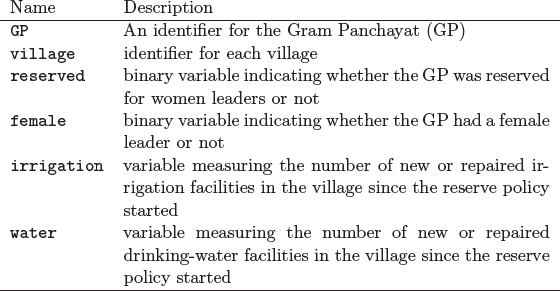
\includegraphics[width=1.0\textwidth]{graphics/women_desc.png}
\end{figure}		

\newpage

\begin{enumerate}
	\item [(a)] State a null and alternative (two-tailed) hypothesis. 
	
	\begin{description}
	  \item [Null] The reservation policy has no effect on the number of new or 
	  repaired drinking water facilities in the villages.
	  \item [Alternate] The reservation policy does have an effect on the number of new or 
	  repaired drinking water facilities in the villages.
	\end{description}
	
	\begin{comment}
	
	The data is as follows: 

| [,3] `reserved`~~ binary variable indicating whether the GP was reserved for women leaders or not
| [,4] `female` ~~binary variable indicating whether the GP had a female leader or not
| [,5] `irrigation` ~~variable measuring the number of new or repaired irrigation facilities in the village since the reserve policy started
| [,6] `water` ~~variable measuring the number of new or repaired drinking-water facilities in the village since the reserve policy started

  \end{comment}
	%\vspace{6cm}

	\item [(b)] Bivariate regression to test this hypothesis:.

  Import the data.

	\lstinputlisting[language=R, firstline=212, lastline=212]{PS02.R}  
	
  \begin{figure}[htb!]
	\caption{\footnotesize{Drinking water projects, grouped by $reserved = [1,0]$}}
	\vspace{.5cm}
	\centering
	\label{fig:water_reserved}
	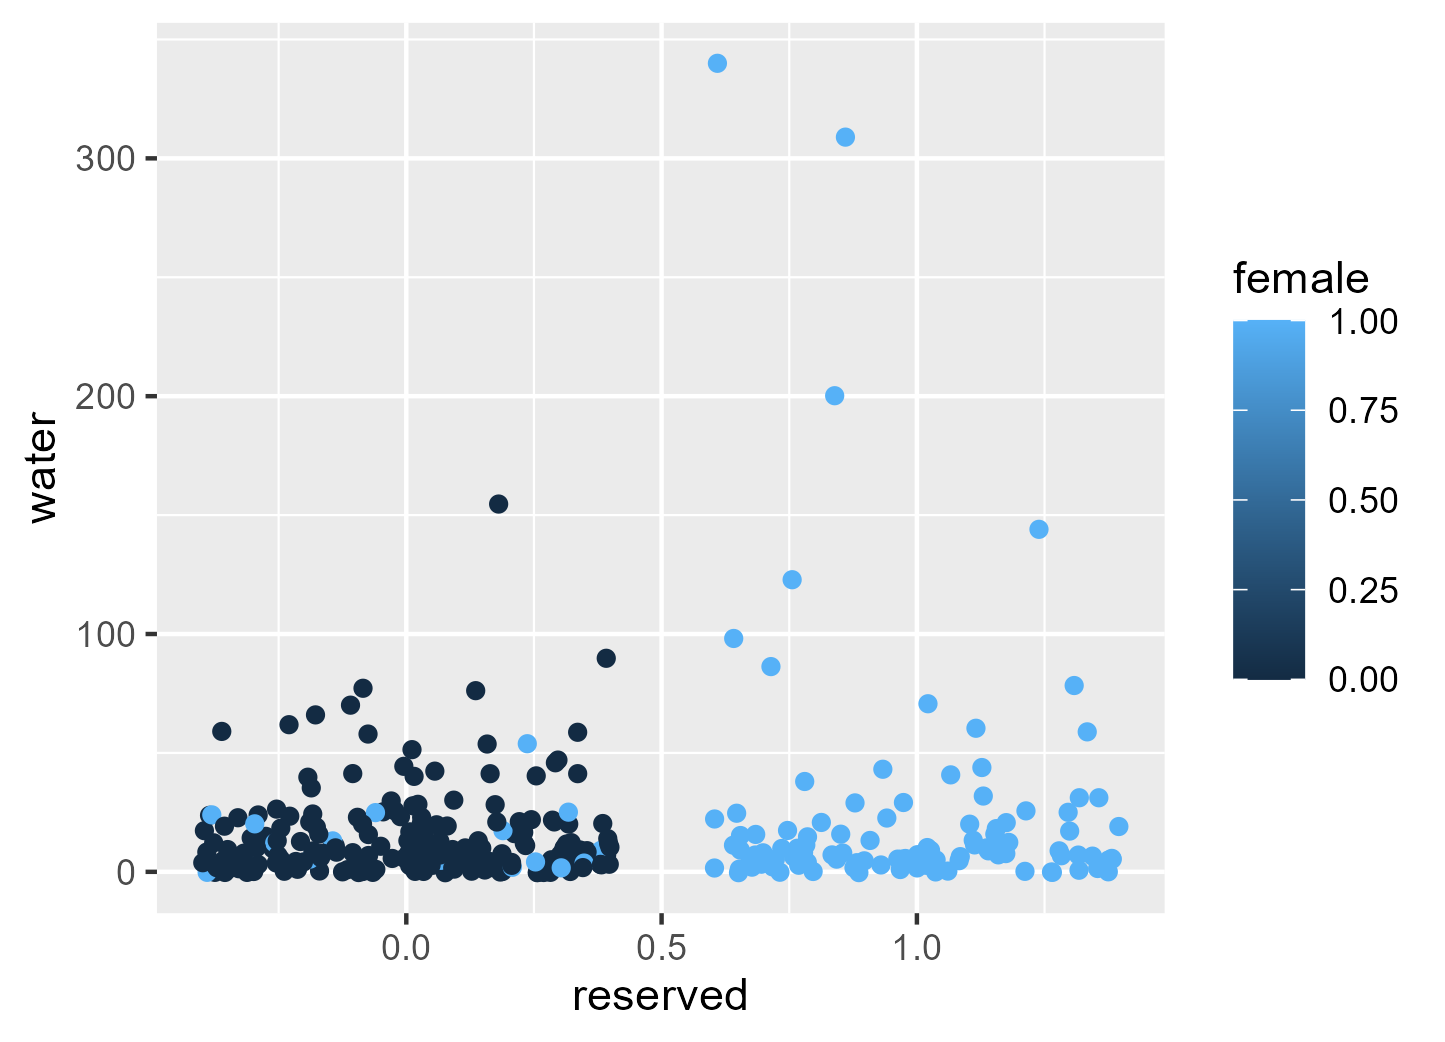
\includegraphics[width=1.0\textwidth]{graphics/resrvd_water.png}
  \end{figure}		
	
	
  The relationship between the 
  \begin{description}
    \item[x = reserved] binary variable indicating whether the GP was reserved for 
  women leaders or not
    \item[y = water] numeric variable denoting the number of new or repaired 
    drinking water facilities in the villages
  \end{description}
  was modelled using the Pearson model for linear regression.  The code is as follows:

	\lstinputlisting[language=R, firstline=229, lastline=268]{PS02.R}  

	This gives the following results:
	
	
% Table created by stargazer v.5.2.3 by Marek Hlavac, Social Policy Institute. E-mail: marek.hlavac at gmail.com
% Date and time: Sat, Oct 15, 2022 - 22:18:21
\begin{table}[htb!] \centering 
  \caption{coefficients for linear regression model water - reserved } 
  \label{tab:coefficients} 
\begin{tabular}{@{\extracolsep{5pt}} ccccc} 
\\[-1.8ex]\hline 
\hline \\[-1.8ex] 
 & estimate  & Std Error & t value & pr(\textgreater \textbar t\textbar ) \\ 
\hline \\[-1.8ex] 
intercept & $14.738$ & $2.286$ & $6.446$ & $4.216474e-10$ \\ 
reserved & $9.252$ & $3.948$ & $2.344$ & $1.970398e-02$ \\ 
\hline \\[-1.8ex] 
\end{tabular} 
\end{table}  

% Table created by stargazer v.5.2.3 by Marek Hlavac, Social Policy Institute. E-mail: marek.hlavac at gmail.com
% Date and time: Sat, Oct 15, 2022 - 22:18:23
\begin{table}[htb] \centering 
  \caption{results for linear regression model water - reserved } 
  \label{tab:results} 
\begin{tabular}{@{\extracolsep{5pt}} cccccc} 
\\[-1.8ex]\hline \\[-1.8ex] 
 & residual error & degrees of freedom & $R\hat{\mkern6mu}2$ & covariance & correlation \\ 
\hline \\[-1.8ex] 
 & 33.4457 & 320 & 0.0169 & 2.0624 & 0.1299 \\ 
\hline \\[-1.8ex] 
\end{tabular} 
\end{table}  


  The estimate for $\beta_0$ is 14.738; the estimate for $\beta_1$ is 9.252, where 
  $y = \beta_0 + \beta_1 * x $; the response variable ($y$) is the incidence of 
  investment in drinking water projects; the explanatory variable ($x$) is 1 if 
  the GP position is reserved for a woman, 0 otherwise.  The pvalue is 0.0197, so 
  at a confidence level of 5\%, we reject the null hypothesis that the two 
  variables are independent.  The $R^2$ value suggests that our model accounts 
  for less than $2\%$ of the variance in our water values.


%	\vspace{6cm}
	\item [(c)] Interpret the coefficient estimate for reservation policy. 

  We expect that where the GP position is not reserved for a female, the average
  number of drinking water projects will be 14.738 and that this will increase by 
  9.252 if the position is reserved.
  
  \end{enumerate}
  
  
\newpage
  \subsection*{Caveats}  
  
  Code in Appendix.
  
  \subsubsection*{Outliers}
	
	On inspection, it is clear that the data, and the model, are significantly affected
	by outliers (see Figure~\ref{fig:reserved_water_boxplot} and Table~\ref{tab:wateroutliers}).
	
  \begin{figure}[htb!]
	\caption{\footnotesize{Boxplot of number of drinking water projects, grouped by reserved}}
	\vspace{.5cm}
	\centering
	\label{fig:reserved_water_boxplot}
	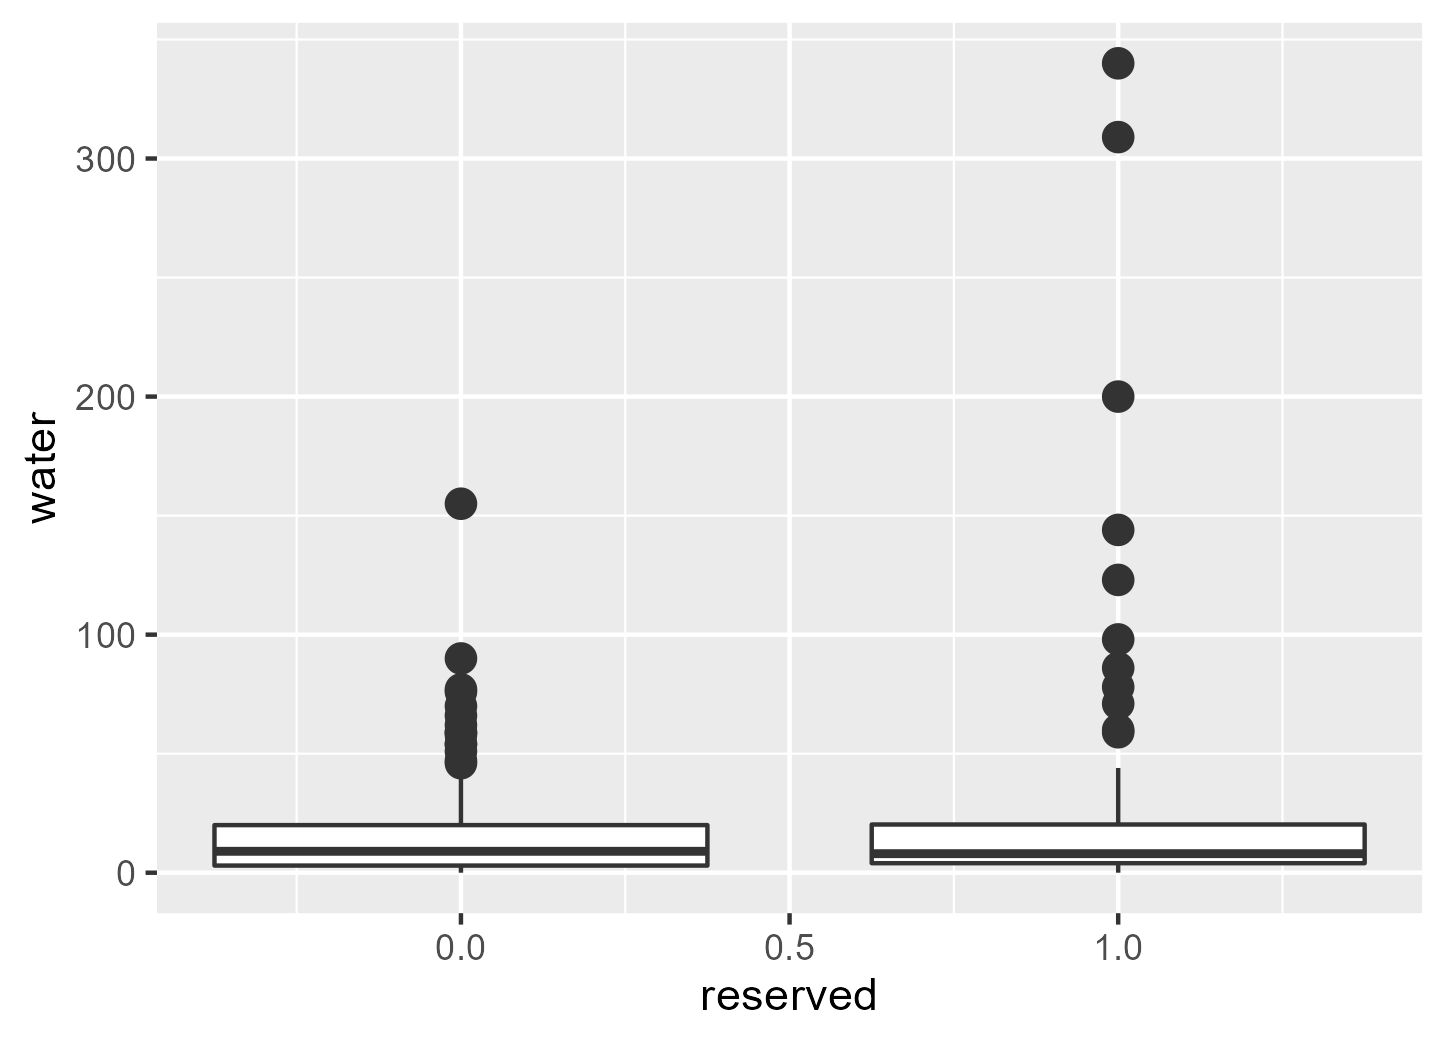
\includegraphics[width=1.0\textwidth]{graphics/resrvd_water_boxplot.png}
  \end{figure}		
	
  
% Table created by stargazer v.5.2.3 by Marek Hlavac, Social Policy Institute. E-mail: marek.hlavac at gmail.com
% Date and time: Thu, Oct 13, 2022 - 19:20:47
\begin{table}[htb] \centering 
  \caption{Outliers in water incidence} 
  \label{tab:wateroutliers} 
\begin{tabular}{@{\extracolsep{5pt}} cccccc} 
\\[-1.8ex]\hline \\[-1.8ex] 
reserved & mean\_water & count\_water & q3 & iqr & outlier\_limit \\ 
\hline \\[-1.8ex] 
0 & 68.267 & 15 & c(`75\%` = 20) & 17 & c(`75\%` = 45.5) \\ 
1 & 142.545 & 11 & c(`75\%` = 20.25) & 16.25 & c(`75\%` = 44.625) \\ 
\hline \\[-1.8ex] 
\end{tabular} 
\end{table}  


  The data was modelled with outliers excluded and the results were as in 
  Table~\ref{tab:noOutliers}
  
  The estimate for $\beta_0$ is 10.7035; the estimate for $\beta_1$ is -0.1571
  (p-value = 0.9015).  Using this data, we cannot reject the hypothesis that 
  water projects and reserved status are independent.  The expected number of 
  drinking water projects decreases by 0.1571 if the village is reserved for a 
  female GP.
  
  However, we have no data to support the idea that the outliers are bad data.  
  We are more likely to conclude that the data is heavily skewed.

  
% Table created by stargazer v.5.2.3 by Marek Hlavac, Social Policy Institute. E-mail: marek.hlavac at gmail.com
% Date and time: Thu, Oct 13, 2022 - 19:20:41
\begin{table}[htb] \centering 
  \caption{Pearson Linear Regression - Water ~ Reserved - excluding outliers} 
  \label{tab:noOutliers} 
\begin{tabular}{@{\extracolsep{5pt}}lc} 
\\[-1.8ex]\hline \\[-1.8ex] 
\\[-1.8ex] & water \\ 
\hline \\[-1.8ex] 
 reserved & $-$0.157 \\ 
  & (1.268) \\ 
  Constant & 10.704$^{***}$ \\ 
  & (0.726) \\ 
 N & 296 \\ 
R$^{2}$ & 0.0001 \\ 
Adjusted R$^{2}$ & $-$0.003 \\ 
Residual Std. Error & 10.243 (df = 294) \\ 
F Statistic & 0.015 (df = 1; 294) \\ 
\hline \\[-1.8ex] 
\multicolumn{2}{l}{$^{*}$p $<$ .1; $^{**}$p $<$ .05; $^{***}$p $<$ .01} \\ 
\end{tabular} 
\end{table}  

  
  \subsubsection*{Villages}
  
  The assumption in using a linear regression model is that each village is a 
  separate case and each case is independent.  However, in this study 
  each GP is associated with two villages, so there is a risk that the values for 
  each village are not independent.
  
  As seen in Figure~\ref{fig:village_boxplot}, the profile for the two sets of data 
  has some differences, mainly the extra high values of the outliers in the 
  $village == 2$ dataset.
  
  \begin{figure}[htb!]
	  \caption{\footnotesize{Drinking water projects, grouped by Village}}
	  \vspace{.5cm}
	  \centering
	  \label{fig:village_boxplot}
	  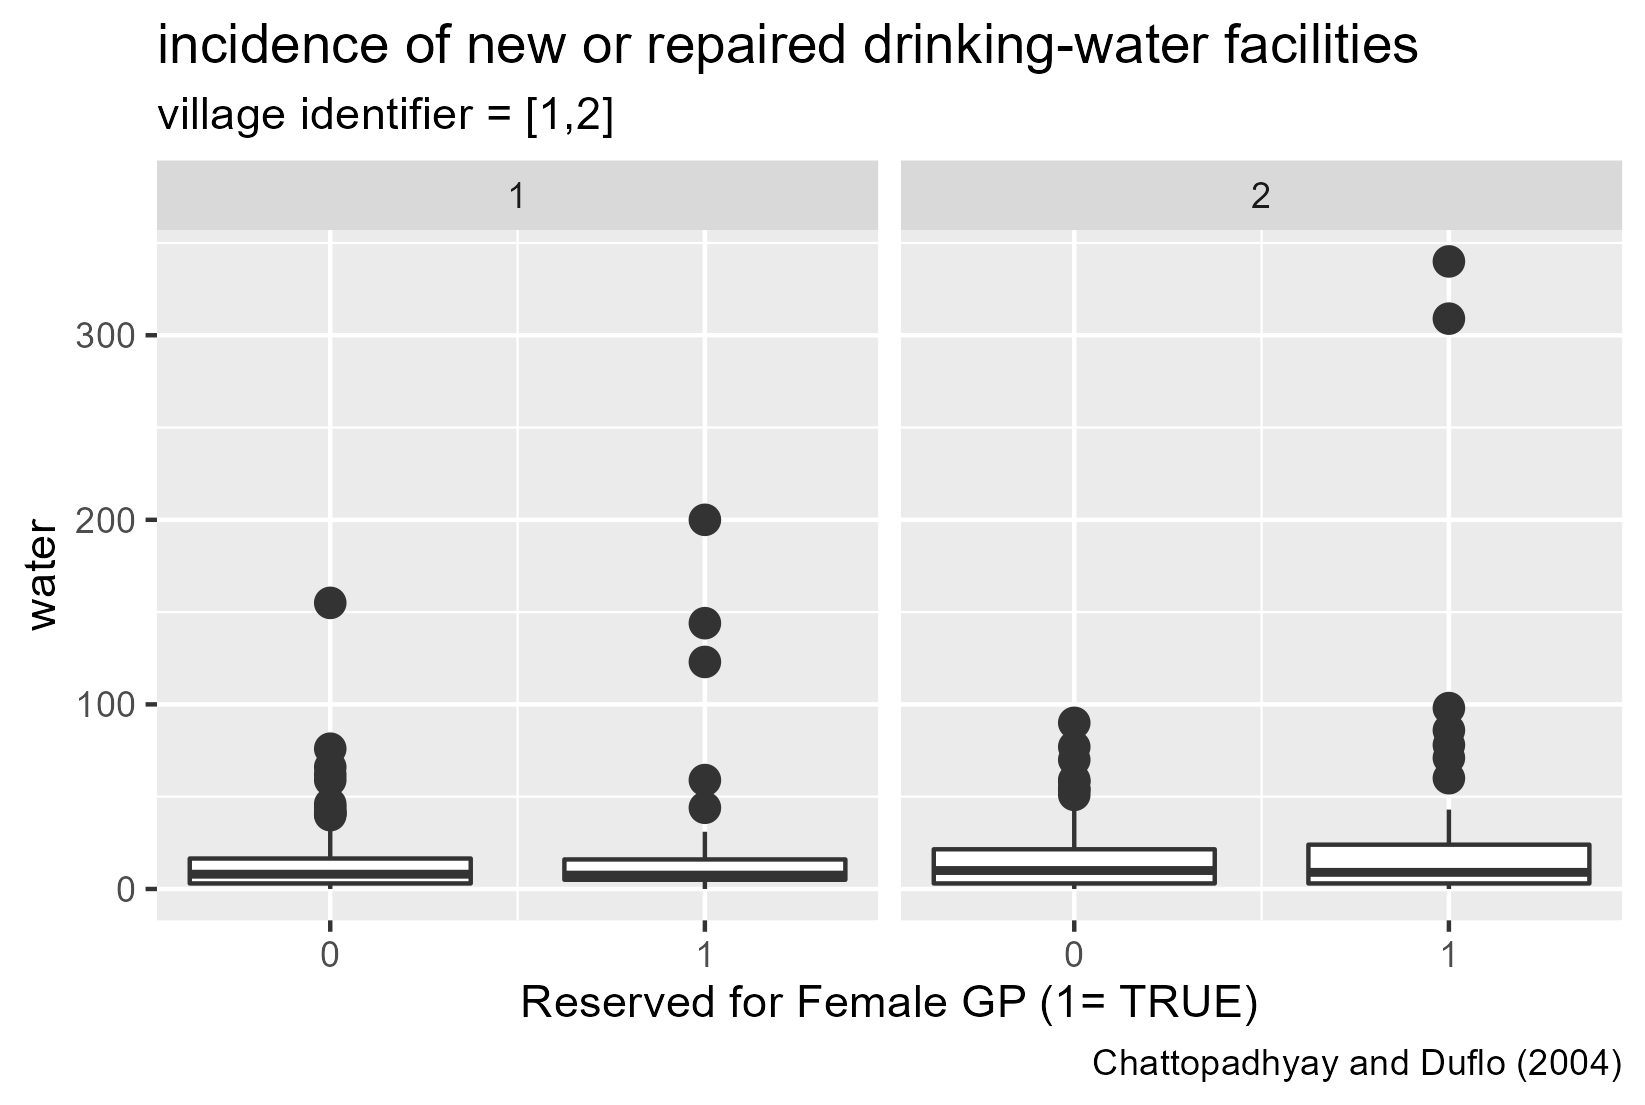
\includegraphics[width=1.0\textwidth]{graphics/village_water_boxplot.png}
  \end{figure}		
	
  A $\chi^2$ test was run on binned values, and this did not reject the hypothesis
  that the two samples were from the same population.
  
  \begin{verbatim}
    	Pearson's Chi-squared test

    data:  one_counts and two_counts
    X-squared = 12, df = 9, p-value = 0.2133
  \end{verbatim}
  
  The linear model with the two villages combined (so our units are now GPs, not 
  villages), gives the same expected values, but with lower confidence as we now 
  have fewer data points.  When the two sets of villages are considered separately
  the estimate for $\beta_1$ is 5.130 for $village==1$ (p-value = 0.2506) and 
  13.374 for $village==2$ (pvalue = 0.04172).
  
  This suggests that splitting or combining our data by village does not add greatly
  to our information about whether $reserved$ is a predictor for $water$. 

  
% Table created by stargazer v.5.2.3 by Marek Hlavac, Social Policy Institute. E-mail: marek.hlavac at gmail.com
% Date and time: Thu, Oct 13, 2022 - 19:19:33
\begin{table}[htb] \centering 
  \caption{Pearson Linear Regression - Water ~ Reserved - Village = 1} 
  \label{tab:village1} 
\begin{tabular}{@{\extracolsep{5pt}}lc} 
\\[-1.8ex]\hline \\[-1.8ex] 
\\[-1.8ex] & water \\ 
\hline \\[-1.8ex] 
 reserved & 5.130 \\ 
  & (4.450) \\ 
  Constant & 13.907$^{***}$ \\ 
  & (2.577) \\ 
 N & 161 \\ 
R$^{2}$ & 0.008 \\ 
Adjusted R$^{2}$ & 0.002 \\ 
Residual Std. Error & 26.656 (df = 159) \\ 
F Statistic & 1.329 (df = 1; 159) \\ 
\hline \\[-1.8ex] 
\multicolumn{2}{l}{$^{*}$p $<$ .1; $^{**}$p $<$ .05; $^{***}$p $<$ .01} \\ 
\end{tabular} 
\end{table}  

% Table created by stargazer v.5.2.3 by Marek Hlavac, Social Policy Institute. E-mail: marek.hlavac at gmail.com
% Date and time: Thu, Oct 13, 2022 - 19:19:34
\begin{table}[htb] \centering 
  \caption{Pearson Linear Regression - Water ~ Reserved - Village = 2} 
  \label{tab:village2} 
\begin{tabular}{@{\extracolsep{5pt}}lc} 
\\[-1.8ex]\hline \\[-1.8ex] 
\\[-1.8ex] & water \\ 
\hline \\[-1.8ex] 
 reserved & 13.374$^{**}$ \\ 
  & (6.515) \\ 
  Constant & 15.570$^{***}$ \\ 
  & (3.773) \\ 
 N & 161 \\ 
R$^{2}$ & 0.026 \\ 
Adjusted R$^{2}$ & 0.020 \\ 
Residual Std. Error & 39.028 (df = 159) \\ 
F Statistic & 4.215$^{**}$ (df = 1; 159) \\ 
\hline \\[-1.8ex] 
\multicolumn{2}{l}{$^{*}$p $<$ .1; $^{**}$p $<$ .05; $^{***}$p $<$ .01} \\ 
\end{tabular} 
\end{table}  

  
  
\newpage
\appendix{Appendix - Code}
	\lstinputlisting[language=R]{PS02.R}  


\end{document}
